\documentclass[12pt,a4paper]{article}
\usepackage[utf8]{inputenc}
\usepackage[turkish]{babel}
\usepackage{amsmath,amssymb,amsfonts,amsthm}
\usepackage{geometry}
\geometry{top=2.5cm,bottom=2.5cm,left=2.5cm,right=2.5cm}
\usepackage{xcolor}
\usepackage{tikz}
\usetikzlibrary{babel}
\usepackage{pgfplots}
\pgfplotsset{compat=1.18}
\usepackage[most]{tcolorbox}
\usepackage{hyperref}
\usepackage{caption}
\usepackage{booktabs}
\usepackage{tabularx}

% -------------------------------------------------
% style.tex – Ortak paketler ve tcolorbox tanımları
% -------------------------------------------------
\usepackage[utf8]{inputenc}
\usepackage[turkish]{babel}
\usepackage{amsmath,amssymb,amsfonts,amsthm}
\usepackage{geometry}
\geometry{top=2.5cm,bottom=2.5cm,left=2.5cm,right=2.5cm}
\usepackage{xcolor}
\usepackage{tikz,pgfplots}
\pgfplotsset{compat=1.18}
\usepackage[most]{tcolorbox}
\usepackage{hyperref}
\usepackage{caption,booktabs,tabularx}

% ---------- Renk tanımları ----------
\definecolor{purp}{RGB}{102,51,153}
\definecolor{tealblue}{RGB}{0,120,130}
\definecolor{mainblue}{RGB}{26,82,118}
\definecolor{alertred}{RGB}{180,40,40}
\definecolor{okgreen}{RGB}{34,139,34}

% ---------- Tek‑argümanlı kutular ----------
\newtcolorbox{box}[2][]{
  colback=white,
  colframe=purp,
  title={#2},
  arc=2mm,
  breakable,
  #1
}

\newtcolorbox{uyari}[1][]{
  colback=yellow!10,
  colframe=orange,
  title={Uyarı},
  arc=2mm,
  breakable,
  #1
}

% ---------- Diğer yardımcı kutular (isteğe bağlı) ----------
\newtcolorbox{ornek}[2][]{
  colback=mainblue!5!white,
  colframe=mainblue,
  title={#2},
  arc=2mm,
  breakable,
  #1
}

\newtcolorbox{odev}[2][]{
  colback=okgreen!5!white,
  colframe=okgreen,
  title={Çözümü Olmayan Ödev ve Tam Çözümü: #2},
  arc=2mm,
  breakable,
  #1
}

\newtcolorbox{tanim}[2][]{
  colback=gray!5!white,
  colframe=gray!60!black,
  title={#2},
  arc=2mm,
  breakable,
  #1
}

\newtcolorbox{sezgi}[2][]{
  colback=tealblue!5!white,
  colframe=tealblue,
  title={Sezgisel Bakış ve Basit Anlatım: #2},
  arc=2mm,
  breakable,
  #1
}

\title{\textbf{İSTATİSTİK TEORİSİ}\\[0.3em] \Large 2. Hafta Ders Notları ve Detaylı Konu Anlatımı}
\author{Ders Notları Düzenlemesi, Sezgisel Açıklamalar ve Çözümlü Analizler}
\date{}

\begin{document}
\maketitle

\begin{abstract}
Bu çalışma; İstatistik Teorisi dersinin 2. haftasında yer alan \textbf{Olasılık Çıkaran Fonksiyon (OÇF / PGF)}, \textbf{Karakteristik Fonksiyon (KF / CF)}, \textbf{Ters Dönüşüm Teoremi (Inversion)}, \textbf{Cauchy Dağılımı}, \textbf{Laplace Dönüşümü} ve \textbf{Kuyruk Olasılığı ile Beklenen Değer Teoremi} konularını içermektedir. Matematiksel ispatların yanında her aracın "neden" geliştirildiği sezgisel benzetmeler ve çözümlü örneklerle ele alınmıştır.
\end{abstract}

\hrule
\vspace{1em}

\section{Büyük Resim: 2. Haftada Ne Öğreniyoruz ve Neden?}

Geçen hafta gördüğümüz Moment Çıkaran Fonksiyon ($M_X(t) = E(e^{tX})$) harika bir araçtı; fakat iki büyük sınırlılığı vardır:
\begin{enumerate}
    \item \textbf{Kesikli Dağılımlarda Olasılıkları Vermez:} MÇF sadece ortalama ve varyans gibi momentleri üretir; doğrudan $P(X=0), P(X=1), P(X=2)$ olasılık değerlerini vermez. Bunun için kesikli değişkenlere özel \textbf{Olasılık Çıkaran Fonksiyon (OÇF)} geliştirilmiştir.
    \item \textbf{Bazı Dağılımlarda MÇF Sonsuza Patlar (Yoktur):} Ağır kuyruklu dağılımlarda (örneğin Cauchy veya $t$-dağılımı) $E(e^{tX})$ integrali ıraksar. Bu krizi çözmek için matematiğin en güçlü silahı olan sanal birim $i = \sqrt{-1}$ devreye sokulur ve \textbf{Karakteristik Fonksiyon} ($\phi(t) = E(e^{itX})$) tanımlanır. Bu fonksiyon istisnasız \textbf{her dağılım için kesinlikle vardır}!
\end{enumerate}

---

\section{Olasılık Çıkaran Fonksiyon (OÇF / PGF)}

\begin{sezgi}{OÇF'nin Basit Mantığı (Olasılıkları Raflara Dizmek)}
Sayma sayıları üzerinde tanımlı kesikli bir değişkenimiz olsun ($X \in \{0, 1, 2, \dots\}$; örneğin bir günde gelen çağrı sayısı, atılan yazı sayısı vb.).  
Bir polinom düşünelim:
\begin{equation}
    g(t) = P(X=0) \cdot t^0 + P(X=1) \cdot t^1 + P(X=2) \cdot t^2 + P(X=3) \cdot t^3 + \dots
\end{equation}
Burada $t$'nin üsleri olayları ($x=0, 1, 2, \dots$), katsayıları ise o olayların olasılıklarını ($P(X=x)$) temsil eden etiketlerdir.  
Biz bu fonksiyona $t=0$ koyup türev alırsak aradığımız olasılık pat diye elimize düşer!
\end{sezgi}

\begin{tanim}{Olasılık Çıkaran Fonksiyon (Probability Generating Function)}
Sayma sayıları üzerinde tanımlı kesikli bir $X$ rastgele değişkeni ($X \in \{0, 1, 2, \dots\}$) için \textbf{Olasılık Çıkaran Fonksiyon} $G_X(t)$ (veya $g(t)$) şu şekilde tanımlanır:
\begin{equation}
    g(t) = G_X(t) = E(t^X) = \sum_{x=0}^{\infty} t^x P(X = x)
\end{equation}
\end{tanim}

\begin{uyari}
\textbf{Terminoloji Düzeltmesi (Sayfa 6):}
El yazısı notların başlığında \textit{"Olasılık Çıkaran Fonksiyon"} yazıldıktan hemen altında parantez içinde İngilizce olarak sehven \textit{"(Moment generating function)"} yazılmıştır.
\begin{itemize}
    \item $E(e^{tX})$ fonksiyonu \textbf{Moment Çıkaran Fonksiyon (MGF / MÇF)}'dir.
    \item $E(t^X)$ fonksiyonu ise \textbf{Olasılık Çıkaran Fonksiyon (PGF / OÇF)}'dir.
    \item İki kavram arasındaki geçiş: $G_X(t) = M_X(\ln t)$ veya $M_X(t) = G_X(e^t)$ şeklindedir.
\end{itemize}
\end{uyari}

\subsection{Olasılık Çıkaran Fonksiyonun 3 Temel Özelliği}
\begin{enumerate}
    \item \textbf{$t=1$'deki Değeri (Toplam Olasılık):}
    \begin{equation}
        g(1) = E(1^X) = \sum_{x=0}^{\infty} P(X = x) = 1
    \end{equation}

    \item \textbf{Olasılıkları Üretme Özelliği ($t=0$'daki Türevler):}
    $g(t)$'nin $k$ kez türevini alıp $t=0$ yazarsak, doğrudan $k$. olasılığı elde ederiz:
    \begin{equation}
        \boxed{P(X = k) = \frac{1}{k!} \left. \frac{d^k g(t)}{dt^k} \right|_{t=0} = \frac{g^{(k)}(0)}{k!}}
    \end{equation}

    \item \textbf{Faktöriyel Momentleri Üretme Özelliği ($t=1$'deki Türevler):}
    $g(t)$'nin $t=1$'deki türevleri ise faktöriyel momentleri verir:
    \begin{equation}
        g'(1) = E(X), \quad g''(1) = E[X(X-1)]
    \end{equation}
    Buradan varyans şu pratik formülle çıkar:
    \begin{equation}
        \boxed{V(X) = g''(1) + g'(1) - [g'(1)]^2}
    \end{equation}
\end{enumerate}

\subsubsection{İspat (Neden $g^{(k)}(0)/k!$ Olasılığı Verir?)}
Polinomu açıkça yazalım:
\begin{equation}
    g(t) = P(X=0) + P(X=1)t + P(X=2)t^2 + P(X=3)t^3 + \dots
\end{equation}
\begin{itemize}
    \item $t=0$ koyarsak: $g(0) = P(X=0)$.
    \item 1. Türev: $g'(t) = P(X=1) + 2P(X=2)t + 3P(X=3)t^2 + \dots \implies g'(0) = 1! P(X=1)$.
    \item 2. Türev: $g''(t) = 2 \cdot 1 P(X=2) + 3 \cdot 2 P(X=3)t + \dots \implies g''(0) = 2! P(X=2)$.
    \item $k$. Türev: $g^{(k)}(0) = k! P(X=k) \implies P(X=k) = \frac{g^{(k)}(0)}{k!}$.
\end{itemize}

\begin{ornek}{Örnek 1: Poisson Dağılımının OÇF ve MÇF'si}
$X \sim \text{Poisson}(\lambda)$ olsun. $X$'in MÇF ve OÇF'sini bulunuz.

\bigskip
\textbf{Çözüm:}
Poisson olasılık kütle fonksiyonu:
\begin{equation}
    P(X = x) = \frac{e^{-\lambda} \lambda^x}{x!}, \quad x = 0, 1, 2, \dots \quad (\lambda > 0)
\end{equation}
\textbf{1. Olasılık Çıkaran Fonksiyon (OÇF):}
\begin{align}
    g(t) = E(t^X) &= \sum_{x=0}^{\infty} t^x \frac{e^{-\lambda} \lambda^x}{x!} = e^{-\lambda} \sum_{x=0}^{\infty} \frac{(\lambda t)^x}{x!} \notag \\
    &= e^{-\lambda} \cdot e^{\lambda t} = \boxed{e^{\lambda(t - 1)}}
\end{align}
\textbf{2. Moment Çıkaran Fonksiyon (MÇF):}  
$t$ yerine $e^t$ yazarak:
\begin{equation}
    M_X(t) = E(e^{tX}) = g(e^t) = \boxed{e^{\lambda(e^t - 1)}}
\end{equation}
\end{ornek}

\begin{uyari}
\textbf{Tanım Kümesi Hatası ve Düzeltmesi (Sayfa 7):}
Notta Poisson dağılımı verilirken tanım kümesi $x > 0$ olarak yazılmıştır. Bu yanlıştır; Poisson dağılımının desteği (support) \textbf{sıfır dahil} tüm negatif olmayan tam sayılardır ($x \in \{0, 1, 2, \dots\}$). Nitekim $P(X=0) = e^{-\lambda} \neq 0$'dır ve serinin başlangıç noktası $x=0$'dır.
\end{uyari}

\begin{center}
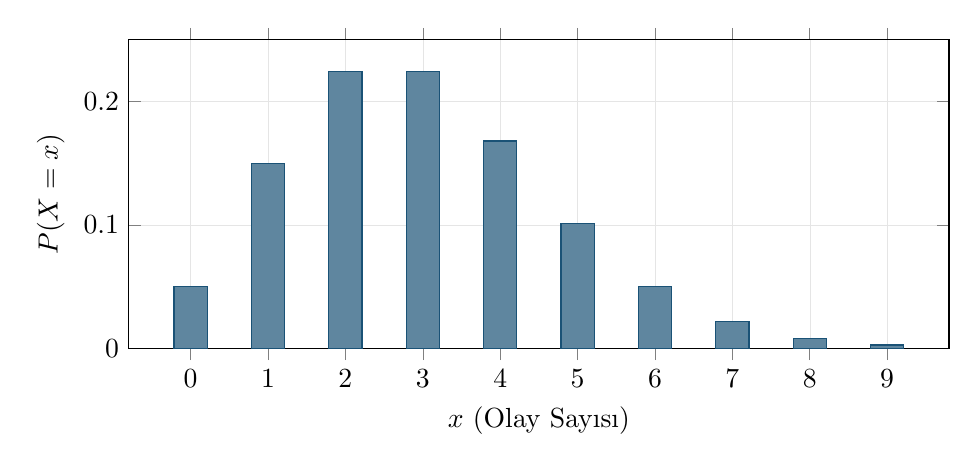
\begin{tikzpicture}
\begin{axis}[
    ybar,
    bar width=12pt,
    width=12cm, height=5.5cm,
    xlabel={$x$ (Olay Sayısı)},
    ylabel={$P(X=x)$},
    ymin=0, ymax=0.25,
    xmin=-0.8, xmax=9.8,
    xtick={0,1,2,3,4,5,6,7,8,9},
    grid=both,
    grid style={line width=.1pt, draw=gray!20}
]
    \addplot[fill=mainblue!70, draw=mainblue] coordinates {
        (0, 0.0498)
        (1, 0.1494)
        (2, 0.2240)
        (3, 0.2240)
        (4, 0.1680)
        (5, 0.1008)
        (6, 0.0504)
        (7, 0.0216)
        (8, 0.0081)
        (9, 0.0027)
    };
\end{axis}
\end{tikzpicture}
\captionof{figure}{$\text{Poisson}(\lambda=3)$ olasılık kütle fonksiyonu. Dağılım $x=0$'da pozitif olasılığa sahiptir ($P(X=0)=e^{-3}\approx 0.05$).}
\end{center}

\vspace{0.5em}
\section{Karakteristik Fonksiyon (KF / CF)}

\begin{sezgi}{Neden Karakteristik Fonksiyon? (MÇF'nin Yetmediği Yer)}
MÇF formülü olan $E(e^{tX}) = \int e^{tx} f(x) dx$ integralinde $t > 0$ iken $x \to \infty$ durumunda $e^{tx}$ üstel olarak devasa hızda büyür. Eğer $f(x)$ fonksiyonu bu büyümeden daha hızlı sönümlenmiyorsa (örneğin Cauchy, $t$-dağılımı veya Pareto gibi kalın kuyruklu dağılımlarda), integral patlar ve MÇF var olmaz!  
İşte matematikçiler burada devreye $i = \sqrt{-1}$ sanal birimini sokmuştur:
\begin{equation}
    |e^{itx}| = |\cos(tx) + i\sin(tx)| = \sqrt{\cos^2(tx) + \sin^2(tx)} = 1
\end{equation}
$e^{itx}$ fonksiyonu reel eksende sonsuza gitmez, sadece birim çember üzerinde döner! Bu sayede integral asla patlamaz.  
\textbf{Altın Kural:} Karakteristik fonksiyon, \textbf{istisnasız her olasılık dağılımı için daima vardır ve $|\phi(t)| \le 1$'dir!}
\end{sezgi}

\begin{tanim}{Karakteristik Fonksiyon (Characteristic Function)}
Bir rastgele değişken $X$ için \textbf{Karakteristik Fonksiyon} $\phi_X(t)$ şu şekilde tanımlanır:
\begin{equation}
    \phi(t) = \phi_X(t) = E(e^{itX}) = 
    \begin{cases}
        \int_{-\infty}^{\infty} e^{itx} f(x) \, dx, & \text{Sürekli ise} \\
        \sum_{x} e^{itx} P(X = x), & \text{Kesikli ise}
    \end{cases}
\end{equation}
Burada $i = \sqrt{-1}$ sanal birimdir. (Bu dönüşüm aslında $f(x)$'in Fourier dönüşümüdür.)
\end{tanim}

\subsection{Karakteristik Fonksiyonun Temel Özellikleri}

\begin{enumerate}
    \item \textbf{Her Dağılım İçin Daima Mevcut ve Sınırlıdır:}
    \begin{equation}
        |\phi(t)| \le \int_{-\infty}^\infty |e^{itx}| f(x) dx = \int_{-\infty}^\infty 1 \cdot f(x) dx = 1
    \end{equation}
    Ayrıca her zaman $\phi(0) = E(e^0) = 1$'dir.

    \item \textbf{Simetrik Dağılımlarda Gerçel (Reel) Olma Özelliği:}
    Eğer $f(x)$ orijine göre simetrik bir fonksiyon ise ($f(-x) = f(x)$), sanal kısım tek fonksiyon olacağından sıfırlanır ve $\phi(t)$ tamamen \textbf{gerçel (reel)} bir fonksiyondur:
    \begin{equation}
        \phi(t) = \int_{-\infty}^{\infty} \cos(tx) f(x) dx + i \underbrace{\int_{-\infty}^{\infty} \sin(tx) f(x) dx}_{0 \text{ (tek fonksiyon)}} = 2 \int_{0}^{\infty} \cos(tx) f(x) dx \in \mathbb{R}
    \end{equation}

    \item \textbf{Doğrusal Dönüşüm:} $Y = a + bX$ ise:
    \begin{equation}
        \phi_Y(t) = e^{ita} \phi_X(bt)
    \end{equation}

    \item \textbf{Momentlerin Üretilmesi:}
    \begin{equation}
        \left. \frac{d^k \phi_X(t)}{dt^k} \right|_{t=0} = i^k E(X^k) \implies \boxed{E(X^k) = (-i)^k \left. \frac{d^k \phi_X(t)}{dt^k} \right|_{t=0}}
    \end{equation}
\end{enumerate}

\subsection{Ters Dönüşüm Teoremi (Inversion Theorem)}
Karakteristik fonksiyon ile olasılık yoğunluk fonksiyonu birbirinin ayna görüntüsüdür. Eğer bir dağılımın $\phi(t)$ karakteristik fonksiyonunu biliyorsanız, orijinal $f(x)$ yoğunluk fonksiyonunu ters Fourier integrali ile kesin olarak bulabilirsiniz:
\begin{equation}
    \boxed{f(x) = \frac{1}{2\pi} \int_{-\infty}^{\infty} e^{-itx} \phi(t) \, dt}
\end{equation}

\begin{ornek}{Örnek 2: $\phi(t) = e^{-t^2/2}$ Fonksiyonundan Yoğunluk Fonksiyonunu Bulma}
$\phi(t) = e^{-t^2/2}$ olan sürekli rastgele değişkenin yoğunluk fonksiyonunu bulunuz.

\bigskip
\textbf{Çözüm:}
Ters dönüşüm formülünü yazalım:
\begin{equation}
    f(x) = \frac{1}{2\pi} \int_{-\infty}^{\infty} e^{-itx} e^{-t^2/2} dt = \frac{1}{2\pi} \int_{-\infty}^{\infty} \exp\left( - \frac{1}{2}(t^2 + 2itx) \right) dt
\end{equation}
Üs kısmını tam kare yapalım: $t^2 + 2itx = (t + ix)^2 - (ix)^2 = (t + ix)^2 + x^2$.  
Yerine koyarsak:
\begin{equation}
    f(x) = \frac{1}{2\pi} e^{-x^2/2} \underbrace{\int_{-\infty}^{\infty} e^{-\frac{1}{2}(t + ix)^2} dt}_{\text{Gauss integrali} = \sqrt{2\pi}} = \frac{\sqrt{2\pi}}{2\pi} e^{-x^2/2} = \boxed{\frac{1}{\sqrt{2\pi}} e^{-x^2/2}}
\end{equation}
Bu standart normal dağılım $X \sim N(0, 1)$'in olasılık yoğunluk fonksiyonudur.
\end{ornek}

\vspace{0.5em}
\section{2. Hafta Ödevi ve Eksiksiz Çözümü}

\begin{odev}{$\phi(t) = e^{-|t|}$ Karakteristik Fonksiyonuna Karşılık Gelen Dağılım}
\textbf{Ödev Sorusu (Sayfa 10):} Bir $X$ rastgele değişkeninin karakteristik fonksiyonu $\phi(t) = e^{-|t|}$ olarak verilmiştir. Bu dağılımın olasılık yoğunluk fonksiyonu $f(x)$'i bulunuz.

\bigskip
\textbf{Adım Adım Çözüm:}
\begin{enumerate}
    \item Ters dönüşüm formülünü uygulayalım:
    \begin{equation}
        f(x) = \frac{1}{2\pi} \int_{-\infty}^{\infty} e^{-itx} e^{-|t|} dt
    \end{equation}
    \item Euler bağıntısını açalım: $e^{-itx} = \cos(tx) - i\sin(tx)$.
    \begin{equation}
        f(x) = \frac{1}{2\pi} \int_{-\infty}^{\infty} \cos(tx) e^{-|t|} dt - \frac{i}{2\pi} \underbrace{\int_{-\infty}^{\infty} \sin(tx) e^{-|t|} dt}_{0 \text{ (tek fonksiyon)}}
    \end{equation}
    \item $\cos(tx) e^{-|t|}$ çift fonksiyon olduğundan $[0, \infty)$ aralığına geçip 2 ile çarpalım:
    \begin{equation}
        f(x) = \frac{1}{2\pi} \cdot 2 \int_{0}^{\infty} \cos(tx) e^{-t} dt = \frac{1}{\pi} \int_{0}^{\infty} e^{-t} \cos(tx) \, dt
    \end{equation}
    \item $J = \int_{0}^{\infty} e^{-t} \cos(tx) dt$ integralini kısmi integrasyon ile hesaplayalım:
    \begin{align}
        u = \cos(tx), \; dv = e^{-t}dt &\implies J = 1 - x \int_0^\infty e^{-t}\sin(tx) dt \\
        \text{Tekrar kısmi integrasyon} &\implies \int_0^\infty e^{-t}\sin(tx) dt = x J \\
        \implies J = 1 - x^2 J &\implies J(1 + x^2) = 1 \implies J = \frac{1}{1 + x^2}
    \end{align}
    \item İntegral sonucunu yerine koyalım:
    \begin{equation}
        \boxed{f(x) = \frac{1}{\pi (1 + x^2)}, \quad -\infty < x < \infty}
    \end{equation}
\end{enumerate}
\textbf{Çok Önemli Teorik Sonuç:} Bu dağılım \textbf{Standart Cauchy Dağılımı}'dır ($X \sim \text{Cauchy}(0,1)$).  
Cauchy dağılımının beklenen değeri ve varyansı yoktur (kuyrukları çok kalındır, $\int |x|f(x)dx = \infty$). Bu nedenle Cauchy'nin Moment Çıkaran Fonksiyonu (MGF) mevcut değildir! Ancak Karakteristik Fonksiyonu $\phi(t) = e^{-|t|}$ sapasağlam mevcuttur.
\end{odev}

\begin{center}
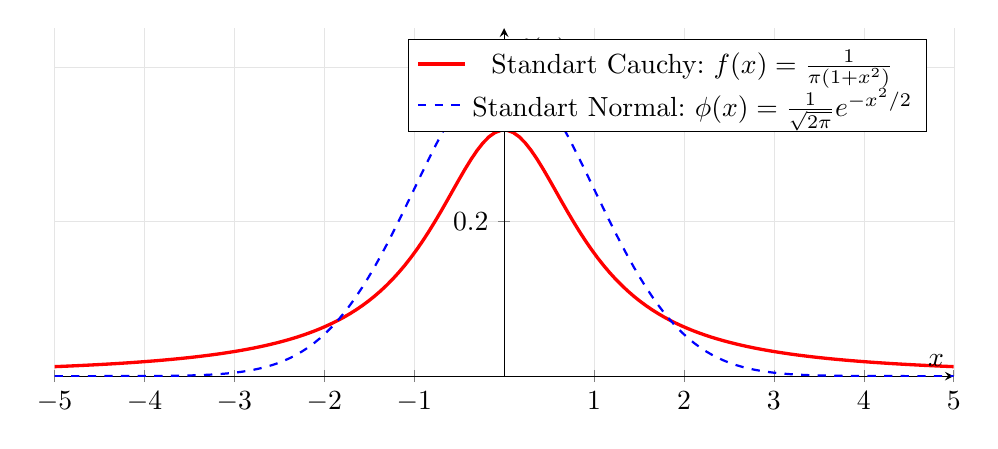
\begin{tikzpicture}
\begin{axis}[
    width=13cm, height=6cm,
    axis lines=center,
    xlabel={$x$}, ylabel={$f(x)$},
    xmin=-5, xmax=5,
    ymin=0, ymax=0.45,
    samples=150,
    domain=-5:5,
    legend pos=north east,
    grid=both,
    grid style={line width=.1pt, draw=gray!20}
]
    % Standart Cauchy: 1 / (pi * (1 + x^2))
    \addplot[red, very thick] {1 / (pi * (1 + x^2))};
    \addlegendentry{Standart Cauchy: $f(x) = \frac{1}{\pi(1+x^2)}$}

    % Standart Normal: 1 / sqrt(2*pi) * exp(-x^2/2)
    \addplot[blue, thick, dashed] {1 / sqrt(2*pi) * exp(-x^2 / 2)};
    \addlegendentry{Standart Normal: $\phi(x) = \frac{1}{\sqrt{2\pi}}e^{-x^2/2}$}
\end{axis}
\end{tikzpicture}
\captionof{figure}{Ödevde bulunan Standart Cauchy dağılımı ile Standart Normal dağılımın karşılaştırması. Cauchy dağılımının kalın kuyrukları (heavy tails) açıkça görülmektedir.}
\end{center}

\vspace{0.5em}
\section{Laplace Dönüşümü ve Kuyruk Beklenen Değer Teoremi}

\begin{tanim}{Laplace Dönüşümü}
Pozitif sürekli rastgele değişkenler ($X \ge 0$) için Laplace dönüşümü:
\begin{equation}
    f^*(s) = \mathcal{L}(f(x)) = E(e^{-sX}) = \int_{0}^{\infty} e^{-sx} f(x) \, dx, \quad (s > 0)
\end{equation}
\end{tanim}

\begin{sezgi}{Kuyruk Olasılığı ile Beklenen Değer (Geometrik Sezgi)}
Genelde $E(X) = \int x f(x) dx$ formülünü biliriz. Fakat $X \ge 0$ olan pozitif değişkenler için (örneğin bir ampulün ömrü, arıza süresi, bekleme süresi):
\begin{equation}
    E(X) = \int_{0}^{\infty} P(X \ge x) \, dx
\end{equation}
şeklinde muhteşem bir alternatif formül vardır!  
\textbf{Anlamı:} Bir cihazın ortalama ömrü ($E(X)$), o cihazın $x$ süresinden fazla hayatta kalma olasılığı fonksiyonunun ($S(x) = 1 - F(x)$) altında kalan toplam alana eşittir.
\end{sezgi}

\begin{ornek}{Örnek 3: Kuyruk Olasılığı Teoreminin İspatı}
$X \ge 0$ sürekli rastgele değişkeni için $E(X) = \int_{0}^{\infty} [1 - F(x)] dx$ olduğunu gösteriniz.

\bigskip
\textbf{Çözüm (Kısmi İntegrasyon İle):}
$u = 1 - F(x) \implies du = -f(x)dx$ ve $dv = dx \implies v = x$ alalım:
\begin{align}
    \int_{0}^{\infty} [1 - F(x)] dx &= \left[ x(1 - F(x)) \right]_{0}^{\infty} - \int_{0}^{\infty} x (-f(x)) dx \notag \\
    &= \left[ \lim_{x \to \infty} x(1 - F(x)) - 0 \right] + \int_{0}^{\infty} x f(x) dx
\end{align}
$E(X) < \infty$ olduğunda sonsuzda $x[1-F(x)] \to 0$ olduğundan sınır terimi sıfırlanır:
\begin{equation}
    \int_{0}^{\infty} P(X \ge x) \, dx = 0 + \int_{0}^{\infty} x f(x) \, dx = \boxed{E(X)}
\end{equation}
\end{ornek}

\begin{center}
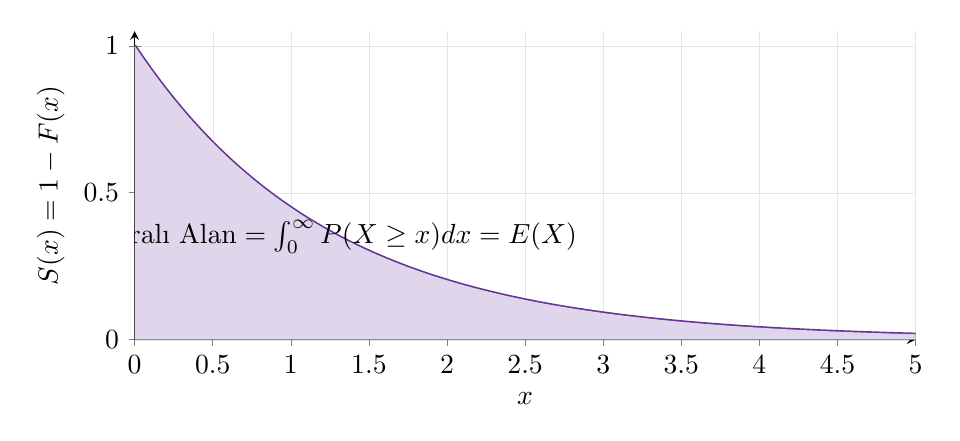
\begin{tikzpicture}
\begin{axis}[
    width=11.5cm, height=5.5cm,
    axis lines=left,
    xlabel={$x$}, ylabel={$S(x) = 1 - F(x)$},
    xmin=0, xmax=5,
    ymin=0, ymax=1.05,
    samples=100,
    domain=0:5,
    grid=both,
    grid style={line width=.1pt, draw=gray!20}
]
    \addplot[purp, very thick] {exp(-0.8*x)};
    \addplot[fill=purp!20, draw=none, domain=0:5] {exp(-0.8*x)} \closedcycle;
    \node at (axis cs:1.3, 0.35) {$\text{Taralı Alan} = \int_0^\infty P(X \ge x) dx = E(X)$};
\end{axis}
\end{tikzpicture}
\captionof{figure}{Kuyruk olasılığı fonksiyonu (Hayatta Kalma / Survival Eğrisi) altındaki alan doğrudan ortalamayı verir.}
\end{center}

\vspace{0.5em}
\section{2. Hafta Hızlı Tekrar ve Dönüşüm Karşılaştırma Tablosu}

\begin{table}[ht]
\centering
\small
\renewcommand{\arraystretch}{1.35}
\begin{tabularx}{\textwidth}{@{}l l l X@{}}
\toprule
\textbf{Dönüşüm} & \textbf{Formül} & \textbf{Tanım Kümesi} & \textbf{Ne İşe Yarar / Temel Üstünlüğü} \\ \midrule
\textbf{OÇF (PGF)} & $G(t) = E(t^X)$ & Kesikli ($X \in \mathbb{N}_0$) & $t=0$'da türev alarak $P(X=k)$ olasılığını verir. \\
\textbf{MÇF (MGF)} & $M(t) = E(e^{tX})$ & Sonlu momentliler & $t=0$'da türev alarak $E(X^k)$ momentlerini üretir. \\
\textbf{Karakteristik (CF)} & $\phi(t) = E(e^{itX})$ & \textbf{Her dağılım} & Her zaman vardır ($|\phi(t)| \le 1$); Cauchy gibi ağır kuyruklarda çalışır. \\
\textbf{Laplace} & $f^*(s) = E(e^{-sX})$ & Pozitif ($X \ge 0$) & Güvenilirlik ve ömür analizlerinde integralleri basitleştirir. \\
\textbf{Kuyruk Teoremi} & $\int_0^\infty P(X \ge x) dx$ & Pozitif ($X \ge 0$) & Yoğunluk yerine hayatta kalma fonksiyonundan $E(X)$ bulur. \\ \bottomrule
\end{tabularx}
\caption{2. Haftada İncelenen Bütün Üreteç ve Dönüşüm Fonksiyonlarının Karşılaştırması}
\end{table}

\end{document}
